\documentclass[conference]{IEEEtran}

\usepackage{cite}
\usepackage{array}
\usepackage{booktabs}
\usepackage{listings}
\usepackage{xcolor}
\usepackage{hyperref}
\usepackage{graphicx}
\usepackage{tikz}
\usetikzlibrary{arrows.meta,positioning,shapes.geometric,fit}

\definecolor{codebg}{RGB}{246,248,252}
\definecolor{codeborder}{RGB}{203,213,225}
\definecolor{verifiedgreen}{RGB}{21,128,61}
\definecolor{unverifiedamber}{RGB}{180,83,9}

\lstset{
    basicstyle=\ttfamily\scriptsize,
    backgroundcolor=\color{codebg},
    frame=single,
    rulecolor=\color{codeborder},
    breaklines=true,
    columns=fullflexible,
    keepspaces=true,
    aboveskip=6pt,
    belowskip=6pt
}

\hypersetup{
    colorlinks=true,
    linkcolor=blue!60!black,
    urlcolor=blue!60!black,
    citecolor=blue!60!black
}

\begin{document}

\title{Private Network Service Platform: Phase 2 High-Availability, Service Isolation, and Failover Evaluation}

\author{
\IEEEauthorblockN{Primary Host Node (\texttt{10.109.112.94}) \quad \& \quad Secondary Host Node — Varun's Mac (\texttt{10.109.112.62})}
\IEEEauthorblockA{Computer Networks Course Project — Private Network Service Platform\\
Private Domains: \texttt{app.team1.test}, \texttt{api.team1.test}\\
\textit{(Insert Student Names / Roll Numbers if required by faculty submission sheet)}}
}

\maketitle

\begin{abstract}
This paper documents the Phase~2 hardening, service isolation, and high-availability failover extensions of the \textit{Private Network Service Platform}, a locally hosted two-Mac Computer Networks system operating over a shared private Wi-Fi LAN without cloud infrastructure. Building on Phase~1 (private \texttt{dnsmasq} resolution, Nginx TLS termination with a local Root CA, round-robin load balancing across two Express.js backends, HTTP caching, and Wireshark packet analysis), Phase~2 introduces a Backup \texttt{dnsmasq} resolver on the Secondary Mac (\texttt{10.109.112.62}), a 30-second DNS TTL (\texttt{local-ttl=30}), macOS Packet Filter (\texttt{pf}) firewall rules isolating backend ports \texttt{4000} and \texttt{6000}, and a Standby Nginx reverse proxy on \texttt{10.109.112.62}. Experimental results verify automatic backup DNS resolution after primary DNS shutdown, uninterrupted backend failover, expected HTTP \texttt{502 Bad Gateway} isolation when both backends stop, PF rule loading with permitted-host access, and successful HTTPS cutover to Standby Nginx serving 8/8 balanced requests (4~Backend~A, 4~Backend~B). Unverified items and architectural constraints---notably process-level rather than machine-level backend redundancy and IP-scoped PF rules---are explicitly disclosed.
\end{abstract}

\begin{IEEEkeywords}
Computer Networks, Private DNS, dnsmasq, Reverse Proxy, Nginx, TLS Termination, Load Balancing, macOS PF Firewall, High Availability, Failover Testing.
\end{IEEEkeywords}

\section{Introduction}
Phase~1 of the \textit{Private Network Service Platform} established a functional local web service pipeline across DNS, TCP, TLS, and HTTP layers using private \texttt{.test} domain names (\texttt{app.team1.test} and \texttt{api.team1.test}), a local Certificate Authority (\texttt{CN\_Project Local Root CA}), an Nginx reverse proxy, and two Express.js REST backends (\texttt{backendA} on port~\texttt{4000} and \texttt{backendB} on port~\texttt{6000}). However, Phase~1 left the Primary Mac (\texttt{10.109.112.94}) as a single point of failure for both DNS resolution and edge TLS termination.

Phase~2 (\textit{Harden \& Recover}) extends the existing two-Mac LAN topology without rebuilding from scratch. By distributing redundant DNS and edge proxy services onto the Secondary Mac (Varun's Mac, \texttt{10.109.112.62}) and enforcing host-level firewall isolation on the Primary Mac (\texttt{10.109.112.94}), Phase~2 validates systematic fault isolation and service continuity under controlled failures.

\section{Phase 2 Objectives}
The Phase~2 engineering effort addresses five core resilience objectives:
\begin{enumerate}
    \item \textbf{Backup DNS Resolver (Extension~A):} Run a secondary \texttt{dnsmasq} instance on \texttt{10.109.112.62} mirroring the project's \texttt{.test} records and verify failover when Primary DNS stops.
    \item \textbf{Controlled DNS TTL (Extension~B):} Configure \texttt{local-ttl=30} across DNS resolvers to limit client-side record caching windows during edge migration.
    \item \textbf{Backend Service Isolation (Extension~C):} Configure macOS Packet Filter (\texttt{pf}) rules on \texttt{10.109.112.94} restricting inbound TCP access on ports \texttt{4000} and \texttt{6000} to loopback and \texttt{10.109.112.62}.
    \item \textbf{High-Availability Backend Failover (Extension~D):} Validate uninterrupted service during single-backend failure, clean \texttt{502 Bad Gateway} behavior when both backends stop, and automatic load-balancing recovery.
    \item \textbf{Controlled Edge Migration (Extension~E):} Deploy Standby Nginx on \texttt{10.109.112.62}, cut over DNS records to \texttt{10.109.112.62}, stop Primary Nginx, and verify balanced HTTPS delivery.
\end{enumerate}

\begin{figure}[t]
\centering
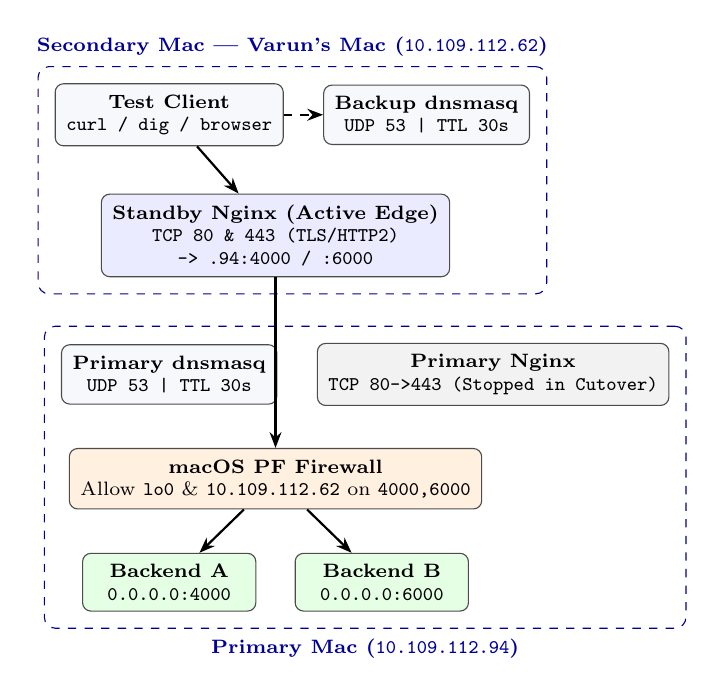
\begin{tikzpicture}[
    node distance=0.55cm and 0.65cm,
    box/.style={rectangle, rounded corners=3pt, draw=black!70, fill=codebg, align=center, font=\scriptsize, inner sep=4pt, minimum width=2.5cm},
    host/.style={rectangle, draw=blue!55!black, dashed, inner sep=6pt, rounded corners=4pt},
    arr/.style={-{Stealth[length=2mm]}, thick}
]
    % Secondary Mac nodes
    \node[box] (client) {\textbf{Test Client}\\ \texttt{curl / dig / browser}};
    \node[box, right=0.5cm of client] (dns2) {\textbf{Backup dnsmasq}\\ \texttt{UDP 53 | TTL 30s}};
    \node[box, below=0.6cm of client, xshift=1.35cm, fill=blue!8] (nginx2) {\textbf{Standby Nginx (Active Edge)}\\ \texttt{TCP 80 \& 443 (TLS/HTTP2)}\\ \texttt{-> .94:4000 / :6000}};

    % Primary Mac nodes
    \node[box, below=0.85cm of nginx2, xshift=-1.35cm] (dns1) {\textbf{Primary dnsmasq}\\ \texttt{UDP 53 | TTL 30s}};
    \node[box, right=0.5cm of dns1, fill=black!5] (nginx1) {\textbf{Primary Nginx}\\ \texttt{TCP 80->443 (Stopped in Cutover)}};
    \node[box, below=0.55cm of dns1, xshift=1.35cm, fill=orange!12] (pf) {\textbf{macOS PF Firewall}\\ Allow \texttt{lo0} \& \texttt{10.109.112.62} on \texttt{4000,6000}};
    \node[box, below=0.55cm of pf, xshift=-1.35cm, fill=green!10, minimum width=2.2cm] (ba) {\textbf{Backend A}\\ \texttt{0.0.0.0:4000}};
    \node[box, below=0.55cm of pf, xshift=1.35cm, fill=green!10, minimum width=2.2cm] (bb) {\textbf{Backend B}\\ \texttt{0.0.0.0:6000}};

    \node[host, fit=(client)(dns2)(nginx2), label={[font=\scriptsize\bfseries, text=blue!60!black]above:Secondary Mac — Varun's Mac (\texttt{10.109.112.62})}] {};
    \node[host, fit=(dns1)(nginx1)(pf)(ba)(bb), label={[font=\scriptsize\bfseries, text=blue!60!black]below:Primary Mac (\texttt{10.109.112.94})}] {};

    \draw[arr, dashed] (client) -- (dns2);
    \draw[arr] (client) -- (nginx2);
    \draw[arr] (nginx2) -- (pf);
    \draw[arr] (pf) -- (ba);
    \draw[arr] (pf) -- (bb);
\end{tikzpicture}
\caption{Two-Mac Phase~2 architecture in active Standby Edge cutover mode.}
\label{fig:arch}
\end{figure}

\section{Backup DNS Implementation}
To eliminate DNS as a single point of failure, a backup \texttt{dnsmasq} server was deployed on the Secondary Mac (\texttt{10.109.112.62}) using Homebrew at \texttt{/opt/homebrew/etc/dnsmasq.conf}. Both \texttt{app.team1.test} and \texttt{api.team1.test} resolve to \texttt{10.109.112.62}, and external queries are forwarded upstream to \texttt{8.8.8.8} and \texttt{1.1.1.1}:

\begin{lstlisting}[caption={Verified Backup \texttt{dnsmasq} Configuration (\texttt{10.109.112.62})}]
listen-address=127.0.0.1,10.109.112.62
bind-interfaces
port=53
no-resolv
server=8.8.8.8
server=1.1.1.1
host-record=app.team1.test,10.109.112.62
host-record=api.team1.test,10.109.112.62
local-ttl=30
log-queries
log-facility=/tmp/dnsmasq-backup.log
\end{lstlisting}

Client resolver settings list the Primary DNS (\texttt{10.109.112.94}) first and Backup DNS (\texttt{10.109.112.62}) second.

\section{DNS TTL Configuration}
Both primary and backup \texttt{dnsmasq} instances enforce \texttt{local-ttl=30} (30~seconds). In production DNS-based traffic steering, a short TTL ensures cached A records expire rapidly so clients pick up updated edge IP addresses during migration.

\textit{Verification Transparency Note:} Although \texttt{local-ttl=30} is configured and verified in the active DNS configuration, a live timed record-change and manual client-side DNS cache-flush (\texttt{dscacheutil -flushcache} / \texttt{killall -HUP mDNSResponder}) demonstration has not yet been confirmed and is marked \textbf{NOT VERIFIED} in Table~\ref{tab:results}.

\section{DNS Failure and Recovery Testing}
Primary \texttt{dnsmasq} on \texttt{10.109.112.94} was intentionally stopped while client DNS settings retained both \texttt{10.109.112.94} and \texttt{10.109.112.62}. Subsequent DNS lookups for \texttt{app.team1.test} and \texttt{api.team1.test} failed over cleanly to the backup resolver on \texttt{10.109.112.62}, returning valid A records. This demonstrates the structural separation between name resolution (UDP port~53) and downstream TCP/HTTPS application delivery.

\section{Backend Firewall Isolation}
In Phase~1, both Express backends bound solely to \texttt{127.0.0.1} on the Primary Mac. To allow the Standby Nginx proxy on \texttt{10.109.112.62} to forward requests across the LAN to ports \texttt{4000} and \texttt{6000}, both running backend processes on \texttt{10.109.112.94} bind to \texttt{0.0.0.0}. To prevent unauthorized LAN clients from bypassing TLS and load balancing, macOS Packet Filter (\texttt{pf}) rules were loaded on \texttt{10.109.112.94}:

\begin{lstlisting}[caption={macOS PF Anchor Rules (\texttt{configs/pf/cn\_project.anchor.conf})}]
pass in quick on lo0 proto tcp from any to any port { 4000, 6000 } keep state
pass in quick proto tcp from 10.109.112.62 to any port { 4000, 6000 } keep state
block in quick proto tcp from any to any port { 4000, 6000 }
\end{lstlisting}

PF rules were loaded and verified on \texttt{10.109.112.94}, confirming that the permitted Secondary Mac (\texttt{10.109.112.62}) can reach both backend ports. Because \texttt{pf} filters at Layer~3/4 (source IP and destination port), the allow rule permits the Secondary Mac host IP (\texttt{10.109.112.62}) rather than exclusively the Nginx process. An independent block test from a third LAN host has not yet been performed (\textbf{NOT VERIFIED}).

\section{Backend Failover Testing}
With Nginx configured for round-robin distribution across Backend~A (\texttt{4000}) and Backend~B (\texttt{6000}), Backend~A was stopped during active traffic. Nginx continued returning HTTP~\texttt{200 OK} responses exclusively from Backend~B (\texttt{X-Backend: B}). When Backend~A was restarted, round-robin alternation between \texttt{X-Backend: A} and \texttt{X-Backend: B} resumed automatically.

\section{Both-Backends-Down Test}
To observe the boundary between the TLS edge proxy and upstream application processes, both Backend~A and Backend~B were stopped simultaneously while DNS and Nginx remained active. Clients still resolved \texttt{app.team1.test}, completed the TCP three-way handshake, and negotiated TLS successfully at Nginx, which then returned \textbf{HTTP \texttt{502 Bad Gateway}}. Restarting both backends immediately restored \textbf{HTTP \texttt{200 OK}} responses.

\section{Standby Nginx Implementation}
A standby Nginx edge reverse proxy was deployed on Varun's Mac (\texttt{10.109.112.62}) at \texttt{\textasciitilde/cn-standby/nginx.conf}, terminating TLS on port~\texttt{443} (with \texttt{http2 on}) using the shared CA-signed server certificate pair (\texttt{app.pem} and \texttt{app-key.pem}) while proxying upstream over the LAN to \texttt{10.109.112.94:4000} and \texttt{10.109.112.94:6000}:

\begin{lstlisting}[caption={Verified Standby Nginx Configuration (\texttt{10.109.112.62})}]
worker_processes 1;
events { worker_connections 1024; }
http {
    upstream backends {
        server 10.109.112.94:4000;
        server 10.109.112.94:6000;
    }
    server {
        listen 80;
        server_name app.team1.test api.team1.test;
        location / {
            proxy_pass http://backends;
            proxy_set_header Host $host;
            proxy_set_header X-Real-IP $remote_addr;
        }
    }
    server {
        listen 443 ssl;
        http2 on;
        server_name app.team1.test api.team1.test;
        ssl_certificate     <STANDBY_CERTS_DIR>/app.pem;
        ssl_certificate_key <STANDBY_CERTS_DIR>/app-key.pem;
        location / {
            proxy_pass http://backends;
            proxy_set_header Host $host;
            proxy_set_header X-Real-IP $remote_addr;
        }
    }
}
\end{lstlisting}

\section{DNS Cutover and HTTPS Verification}
To validate edge migration, both primary and backup \texttt{dnsmasq} resolvers were updated to return \texttt{10.109.112.62} for \texttt{app.team1.test} and \texttt{api.team1.test}, and Primary Nginx on \texttt{10.109.112.94} was stopped. HTTPS requests from the client succeeded without certificate warnings after trusting \texttt{certs/rootCA.pem} (\texttt{CN=CN\_Project Local Root CA}) in the macOS System Keychain, proving seamless TLS identity portability across edge hosts.

\section{Standby Load-Balancing Results}
Following the DNS cutover to \texttt{10.109.112.62} and shutdown of Primary Nginx, eight consecutive HTTPS requests were executed against Standby Nginx. All eight requests succeeded (\textbf{8/8 HTTP \texttt{200 OK}}), distributed evenly with \textbf{4 responses from Backend~A} (\texttt{X-Backend: A}) and \textbf{4 responses from Backend~B} (\texttt{X-Backend: B}).

\section{Troubleshooting and Observations}
\begin{itemize}
    \item \textbf{Loopback vs.\ LAN Backend Binding:} Committed repository files (\texttt{backendA/server.js} and \texttt{backendB/server.js}) retain Phase~1 \texttt{127.0.0.1} binding, whereas Phase~2 cross-Mac standby proxying requires \texttt{0.0.0.0} binding paired with PF firewall rules on \texttt{10.109.112.94}.
    \item \textbf{Layer-Isolated Error Signatures:} DNS misrouting (demonstrated earlier in Phase~1 diagnostics using unreachable \texttt{.250}) breaks connectivity prior to TCP, whereas dual-backend failure yields TLS success followed by HTTP~\texttt{502 Bad Gateway}.
    \item \textbf{HTTP Caching Verification:} Endpoint \texttt{/api/cached} consistently sets \texttt{Cache-Control: public, max-age=60} and \texttt{ETag: "v1"}, returning \texttt{304 Not Modified} on conditional requests.
\end{itemize}

\begin{table*}[t]
\centering
\caption{Phase 1 & Phase 2 Verification Matrix}
\label{tab:results}
\renewcommand{\arraystretch}{1.18}
\begin{tabular}{@{}cl p{4.0cm} p{3.5cm} p{4.2cm} c@{}}
\toprule
\textbf{ID} & \textbf{Test Case} & \textbf{Procedure} & \textbf{Expected Result} & \textbf{Actual Verified Result} & \textbf{Status} \\
\midrule
T1 & Two-Mac LAN Connectivity & Connect \texttt{.94} \& \texttt{.62} on same Wi-Fi LAN; run \texttt{ping} & Bidirectional ICMP replies & Both Macs communicate cleanly over the same LAN & \textcolor{verifiedgreen}{\textbf{VERIFIED}} \\
T2 & Primary \& Backup DNS & Query \texttt{app.team1.test} \& \texttt{api.team1.test} on \texttt{.94} and \texttt{.62} & Both return A record (\texttt{10.109.112.62}) & Both \texttt{dnsmasq} services resolve both private domains & \textcolor{verifiedgreen}{\textbf{VERIFIED}} \\
T3 & DNS TTL Configuration & Inspect \texttt{local-ttl} directive in \texttt{dnsmasq} config & TTL set to 30 seconds & \texttt{local-ttl=30} configured in primary \& backup DNS & \textcolor{verifiedgreen}{\textbf{VERIFIED}} \\
T4 & Primary DNS Failure & Stop primary \texttt{dnsmasq} on \texttt{.94}; query domains & Client fails over to backup DNS \texttt{.62} & Backup resolver resolved domains after primary stopped & \textcolor{verifiedgreen}{\textbf{VERIFIED}} \\
T5 & DNS Record Change \& Flush & Alter record; observe 30s TTL cache \& manual flush & Old IP cached until TTL or \texttt{dscacheutil} flush & Timed change \& client flush demo not yet confirmed & \textcolor{unverifiedamber}{\textbf{NOT VERIFIED}} \\
T6 & Backend A \& B Responses & Query \texttt{4000} and \texttt{6000} endpoints & Both return \texttt{200 OK} + \texttt{X-Backend} & Backend~A and Backend~B respond successfully & \textcolor{verifiedgreen}{\textbf{VERIFIED}} \\
T7 & Nginx Load Balancing & Send repeated requests through Nginx edge & Alternating \texttt{X-Backend: A/B} & Nginx distributes requests across Backend~A and B & \textcolor{verifiedgreen}{\textbf{VERIFIED}} \\
T8 & Trusted HTTPS Validation & Trust \texttt{rootCA.pem}; access \texttt{https://app.team1.test} & Valid TLS chain without \texttt{-k} bypass & HTTPS certificate validation succeeds after trusting CA & \textcolor{verifiedgreen}{\textbf{VERIFIED}} \\
T9 & HTTP Caching (\texttt{ETag}/\texttt{304}) & Request \texttt{/api/cached}, then \texttt{If-None-Match: "v1"} & \texttt{ETag: "v1"} and \texttt{304 Not Modified} & \texttt{/api/cached} supports ETag and HTTP \texttt{304} responses & \textcolor{verifiedgreen}{\textbf{VERIFIED}} \\
T10 & Single-Backend Failover & Stop Backend~A; test edge; restart Backend~A & Continues via B; LB resumes on restart & Stopping A serves via B; restart restores LB & \textcolor{verifiedgreen}{\textbf{VERIFIED}} \\
T11 & Both-Backends-Down & Stop A \& B; request edge; restart both & Returns \texttt{502}; restart restores \texttt{200} & Stopping both gave HTTP \texttt{502}; restart restored \texttt{200} & \textcolor{verifiedgreen}{\textbf{VERIFIED}} \\
T12 & PF Load \& \texttt{.62} Access & Load PF anchor on \texttt{.94}; probe \texttt{4000}/\texttt{6000} from \texttt{.62} & PF loaded; \texttt{.62} reaches both ports & PF loaded and verified; \texttt{.62} reached both ports & \textcolor{verifiedgreen}{\textbf{VERIFIED}} \\
T13 & PF Block Third LAN Host & Probe \texttt{.94:4000}/\texttt{6000} from non-\texttt{.62} host & Inbound TCP dropped by PF & Independent third-host drop test not yet executed & \textcolor{unverifiedamber}{\textbf{NOT VERIFIED}} \\
T14 & Standby Nginx Cutover & Stop Primary Nginx on \texttt{.94}; request via DNS & Standby Nginx on \texttt{.62} serves HTTPS & Standby Nginx served application after primary stopped & \textcolor{verifiedgreen}{\textbf{VERIFIED}} \\
T15 & Standby LB Distribution & Send 8 HTTPS requests to Standby Nginx (\texttt{.62}) & Balanced \texttt{200 OK} across A \& B & 8/8 HTTPS \texttt{200 OK}: 4~Backend~A, 4~Backend~B & \textcolor{verifiedgreen}{\textbf{VERIFIED}} \\
\bottomrule
\end{tabular}
\end{table*}

\section{Limitations}
\begin{enumerate}
    \item \textbf{Process-Level vs.\ Machine-Level Backend Redundancy:} Both Backend~A (\texttt{4000}) and Backend~B (\texttt{6000}) execute on the same Primary Mac (\texttt{10.109.112.94}). Consequently, backend failover provides \textbf{process-level redundancy only}; a full hardware, power, or Wi-Fi failure on \texttt{10.109.112.94} takes both backends offline simultaneously.
    \item \textbf{IP-Scoped PF Firewall Rule:} The macOS PF allow rule authorizes source IP \texttt{10.109.112.62} rather than authenticating the remote Nginx process, meaning any tool running on the Secondary Mac can connect to ports \texttt{4000} and \texttt{6000}.
    \item \textbf{Manual Edge Cutover \& Unverified Items:} DNS record cutover is manual, Standby Nginx omits primary's port~80 redirect and passive \texttt{max\_fails} directives, and tests T5 and T13 remain \textbf{NOT VERIFIED}.
\end{enumerate}

\section{Conclusion}
Phase~2 successfully hardened the \textit{Private Network Service Platform} across two macOS hosts. Backup \texttt{dnsmasq}, Standby Nginx TLS termination, PF backend isolation, and systematic failover testing eliminated single points of failure at the DNS and reverse-proxy edge layers while accurately bounding process-level backend redundancy and open verification items.

\end{document}
